\documentclass{beamer}

\mode<presentation>
{
  \usetheme{default}      % or try Darmstadt, Madrid, Warsaw, ...
  \usecolortheme{default} % or try albatross, beaver, crane, ...
  \usefonttheme{default}  % or try serif, structurebold, ...
  \setbeamertemplate{navigation symbols}{}
  \setbeamertemplate{caption}[numbered]
  \setbeamerfont{page number in head/foot}{size=\large}
  \setbeamertemplate{footline}[frame number]

}

\usepackage[english]{babel}
\usepackage[utf8x]{inputenc}
\usepackage{hyperref}
\usepackage{color}
\usepackage{epigraph}
\usepackage[procnames]{listings}
\usepackage{textcomp}
\usepackage{setspace}
\usepackage{palatino}
\renewcommand{\lstlistlistingname}{Code Listings}
\renewcommand{\lstlistingname}{Code Listing}
\definecolor{gray}{gray}{0.5}
\definecolor{green}{rgb}{0,0.5,0}
\definecolor{lightgreen}{rgb}{0,0.7,0}
\definecolor{purple}{rgb}{0.5,0,0.5}
\definecolor{darkred}{rgb}{0.5,0,0}
\lstnewenvironment{python}[1][]{
\lstset{
language=python,
basicstyle=\ttfamily\scriptsize\setstretch{1},
stringstyle=\color{green},
showstringspaces=false,
alsoletter={1234567890},
otherkeywords={\ , \}, \{},
keywordstyle=\color{blue},
emph={access,and,as,break,class,continue,def,del,elif,else,%
except,exec,finally,for,from,global,if,import,in,is,%
lambda,not,or,pass,print,raise,return,try,while,assert},
emphstyle=\color{orange}\bfseries,
emph={[2]self},
emphstyle=[2]\color{gray},
emph={[4]ArithmeticError,AssertionError,AttributeError,BaseException,%
DeprecationWarning,EOFError,Ellipsis,EnvironmentError,Exception,%
False,FloatingPointError,FutureWarning,GeneratorExit,IOError,%
ImportError,ImportWarning,IndentationError,IndexError,KeyError,%
KeyboardInterrupt,LookupError,MemoryError,NameError,None,%
NotImplemented,NotImplementedError,OSError,OverflowError,%
PendingDeprecationWarning,ReferenceError,RuntimeError,RuntimeWarning,%
StandardError,StopIteration,SyntaxError,SyntaxWarning,SystemError,%
SystemExit,TabError,True,TypeError,UnboundLocalError,UnicodeDecodeError,%
UnicodeEncodeError,UnicodeError,UnicodeTranslateError,UnicodeWarning,%
UserWarning,ValueError,Warning,ZeroDivisionError,abs,all,any,apply,%
basestring,bool,buffer,callable,chr,classmethod,cmp,coerce,compile,%
complex,copyright,credits,delattr,dict,dir,divmod,enumerate,eval,%
execfile,exit,file,filter,float,frozenset,getattr,globals,hasattr,%
hash,help,hex,id,input,int,intern,isinstance,issubclass,iter,len,%
license,list,locals,long,map,max,min,object,oct,open,ord,pow,property,%
quit,range,raw_input,reduce,reload,repr,reversed,round,set,setattr,%
slice,sorted,staticmethod,str,sum,super,tuple,type,unichr,unicode,%
vars,xrange,zip},
emphstyle=[4]\color{purple}\bfseries,
upquote=true,
morecomment=[s][\color{lightgreen}]{"""}{"""},
commentstyle=\color{red}\slshape,
literate={>>>}{\textbf{\textcolor{darkred}{>{>}>}}}3%
         {...}{{\textcolor{gray}{...}}}3,
procnamekeys={def,class},
procnamestyle=\color{blue}\textbf,
framexleftmargin=1mm, framextopmargin=1mm, frame=shadowbox,
rulesepcolor=\color{blue},#1
}}{}


\lstset{basicstyle=\small}

\linespread{1.1}

\title[The \texttt{clld} toolkit]{The \texttt{clld} toolkit}
\author{Robert Forkel and Sebastian Bank}
\institute{Max Planck Institute for Evolutionary Anthropology, Leipzig}
\date{October 7, 2014}

\begin{document}
\begin{frame}
  \titlepage
\end{frame}

% Uncomment these lines for an automatically generated outline.
\begin{frame}{Outline}
%Presentation puts focus on cross-liguistic data from
%the perspective of data re-use.

% paper does also talk about perspective of data creators.
  \tableofcontents
\end{frame}

\section{The CLLD project}

\begin{frame}{The CLLD project: Overview}
Funded by the Max Planck Society for 4 years.
\vskip 0.5cm
Creates infrastructure for publishing cross-linguistic datasets, including
\begin{itemize}
\item organization: a publication platform \texttt{\textbf{http://clld.org}} supporting two publication models:
\begin{itemize}
\item Standalone databases following an "edited series" model, like WALS, WOLD, \dots
\item Two journals for cross-linguistic datasets
\end{itemize}
\item infrastructure: Glottolog, a language catalog and comprehensive bibliography
\item technology: the \texttt{clld} toolkit powering our applications
\end{itemize}
\end{frame}

\begin{frame}{The CLLD project: Datasets}
Typological:
\begin{itemize}
\item \href{http://wals.info}{WALS} -
{\scriptsize the World Atlas of Language Structures - a database of structural properties of more than 2600 languages}
\item \href{http://apics-online.info}{APiCS} -
{\scriptsize the Atlas of Pidgin and Creole Language Structures}
\item \href{http://sails.clld.org}{SAILS} -
{\scriptsize the South American Indigenous Language Structures}
\item \href{http://phoible.org}{PHOIBLE} -
{\scriptsize a repository of cross-linguistic phonological inventory data}
%\item Typological: eWAVE
\end{itemize}
Lexical:
\begin{itemize}
\item \href{http://wold.clld.org}{WOLD} -
{\scriptsize the World Loanword Database contains vocabularies of 41 languages from around the world annotated for loanword status}
\item \href{http://tsammalex.clld.org}{Tsammalex} -
{\scriptsize a multilingual lexical database on plants and animals}
\item \href{http://lingweb.eva.mpg.de/ids/}{IDS} -
{\scriptsize the Intercontinental Dictionary Series (to be published in CLLD in 2014)}
\item ASJP -
{\scriptsize the Automated Similarity Judgement Project (to be published in 2014)}
\end{itemize}
Encyclopedic:
\begin{itemize}
\item \href{http://glottolog.org}{Glottolog} -
{\scriptsize a language catalog and comprehensive bibliography}
\end{itemize}
\end{frame}


%
% TODO: screenshots!
%
\begin{frame}{The CLLD project: WALS}
\begin{figure}
\includegraphics[width=0.7\textwidth]{wals.png}
\end{figure}
\end{frame}

\begin{frame}{The CLLD project: WOLD}
\begin{figure}
\includegraphics[width=0.7\textwidth]{wold.png}
\end{figure}
\end{frame}

\begin{frame}{The CLLD project: APiCS}
\begin{figure}
\includegraphics[width=0.7\textwidth]{apics2.png}
\end{figure}
\end{frame}

\begin{frame}{The CLLD project: Glottolog}
\begin{figure}
\includegraphics[width=0.7\textwidth]{glottolog.png}
\end{figure}
\end{frame}

\begin{frame}{The CLLD project: AfBo}
\begin{figure}
\includegraphics[width=0.7\textwidth]{afbo.png}
\end{figure}
\end{frame}

\begin{frame}{The CLLD project: eWAVE}
\begin{figure}
\includegraphics[width=0.7\textwidth]{ewave.png}
\end{figure}
\end{frame}

\begin{frame}{The CLLD project: SAILS}
\begin{figure}
\includegraphics[width=0.7\textwidth]{sails.png}
\end{figure}
\end{frame}

\begin{frame}{The CLLD project: PHOIBLE}
\begin{figure}
\includegraphics[width=0.7\textwidth]{phoible.png}
\end{figure}
\end{frame}

\begin{frame}{The CLLD project: Tsammalex}
\begin{figure}
\includegraphics[width=0.7\textwidth]{tsammalex.png}
\end{figure}
\end{frame}


\begin{frame}[fragile]{The CLLD project: Where's my dataset?}
Have a dataset in need of publication and presentation on the web?
\begin{itemize}
\item Submit to Harald's \textbf{J}ournal of \textbf{C}ross-\textbf{L}inguistic \textbf{D}atabases or
\item submit to Martin's edited series of cross-linguistic databases \textbf{clld.org} or
\item get a seasoned python programmer for a month to build your own app on top of the
\texttt{clld} toolkit!
\lstinputlisting[basicstyle=\ttfamily\tiny]{phoible_cloc.txt}
\end{itemize}
\end{frame}

\section{The \texttt{clld} toolkit}

\begin{frame}{The \texttt{clld} toolkit: Motivation}
\begin{quote}
Survey databases are all alike.
\end{quote}
Can we extract functionality needed to build WALS, WOLD, and APiCS into a reusable
piece of software?

Design goals:
\begin{itemize}
\item There must be a core database model, which allows for as much shared
functionality as possible.
%\item Deployment of applications must be uniform and easy.
\item User interfaces of applications must be fully customizable.
\item It must be easy to re-implement legacy applications using the framework.
\item Optimize for maintainability, i.e.~minimize lines-of-code for apps built
with the framework.
\item Find the right level of abstraction!
\end{itemize}
\end{frame}


\begin{frame}{\texttt{clld}: A CMS for cross-linguistic data}
The \texttt{clld} toolkit is an open source Python package
hosted on \href{https://github.com/clld/clld}{GitHub}
providing
\begin{itemize}
\item an extensible core data model
\item a web application framework
\begin{itemize}
\item powering all CLLD databases
\item providing a basic API built on Linked Data principles
\item "reference implementation" of a dataset browser
\item \texttt{clld} apps are web applications built as small layer of code on top
of the \texttt{clld} framework.
\item \texttt{clld} works with python 2.7 and 3.4 and has a test suite with
100\% coverage.
\end{itemize}
%\item utilities
\end{itemize}
%Remainder of talk will explore what's built-in the core and how to extend
%the framework.
\end{frame}


\begin{frame}{Intermezzo: Disambiguation}
\begin{itemize}
\item {\color{darkred}CLLD}: The project.
\item {\color{darkred}clld.org}: The publisher/brand.
\item {\color{darkred}\texttt{clld}}: The software, aka toolkit, aka framework.
\item {\color{darkred}\texttt{clld} app}: A web application built using the \texttt{clld} framework.
\end{itemize}
In the remainder of this presentation we will talk about the latter two.
\end{frame}


\subsection{The data model}

\begin{frame}{\texttt{clld} data model: Design}
The design of the data model was guided by three principles:
\begin{itemize}
\item All the target datasets have to “fit in” without loss.
\item The data model must be as abstract as necessary, as concrete as possible.
\item The data model must be extensible.
\end{itemize}
\end{frame}


\begin{frame}{\texttt{clld} data model: Entities}
\begin{itemize}
\item {\color{darkred}Dataset} {\scriptsize holds metadata about a dataset like license and publisher information.}
\item {\color{darkred}Language} {\scriptsize may be a languoid (Glottolog) or doculect (ASJP).}
\item {\color{darkred}Parameter} {\scriptsize a feature that can be determined and coded for a language – e.g.~a
word meaning, or a typological feature.}
\item {\color{darkred}ValueSet} {\scriptsize set of values
measured/observed/recorded for one language and one parameter,
i.e.~the points in the Language-Parameter-matrix.}
\item {\color{darkred}Value} {\scriptsize a single measurement (different types of scales
can be modeled using custom attributes).
% TODO: example: nominal/enumerated/ordinal
}
\item {\color{darkred}Unit} {\scriptsize parts of a language system that are annotated, such as sounds, words or constructions.}
\item {\color{darkred}UnitParameter} {\scriptsize a feature that can be determined for a unit.}
\item {\color{darkred}UnitValue} {\scriptsize measurement for one unit and one unitparameter.}
%\item {\color{darkred}Source} {\scriptsize pointer to secondary literature – e.g. a bibliographical record.}
%\item {\color{darkred}Sentence} {\scriptsize a small piece of text, preferably in the form of interlinear glossed text according to the Leipzig Glossing Rules.}
\item {\color{darkred}Contribution} {\scriptsize ValueSets can be partitioned into separate contributions sharing provenance.}
\end{itemize}
\end{frame}



\begin{frame}{\texttt{clld} data model: Relationships}
\begin{figure}
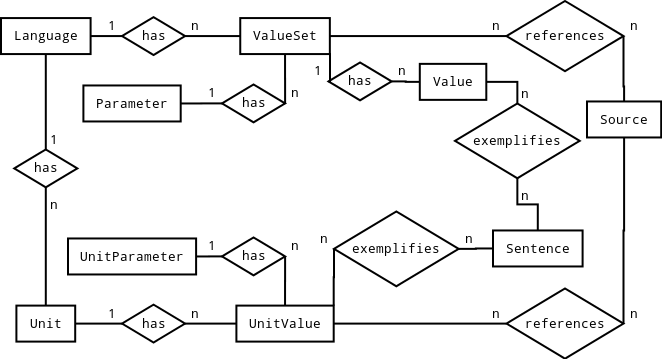
\includegraphics[width=0.9\textwidth]{clld_erd.png}
\caption{\label{fig:clld}The default \texttt{clld} data model.
Note: Modelling constructions as Units and features as UnitParameters the case
mentioned by Harald fits in.}
\end{figure}
\end{frame}


\begin{frame}[fragile]{\texttt{clld} data model: Extensibility}
\texttt{clld} uses \textit{joined table inheritance} as implemented in
SQLAlchemy to provide extensibility of the core data model:
\begin{itemize}
\item Each core model can be specialised/customized in a \texttt{clld} app,
adding columns or relationships.
\begin{python}
@implementer(ILanguage)
class Languoid(Language, CustomModelMixin):
    ...
\end{python}
\item The ORM (Object Relational Mapper) transparently joins the two
corresponding tables when querying, retrieving the specialized object,
i.e.~the full set of columns.
\item Additional models can be added freely, reusing \texttt{clld} functionality
to enable functionality like versioning, etc.
\end{itemize}
\end{frame}


\begin{frame}[fragile]{\texttt{clld} data model: Lexical data}
\begin{figure}
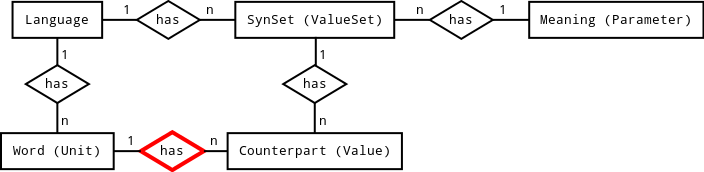
\includegraphics[width=\textwidth]{wold_erd.png}
\caption{\label{fig:wold}The WOLD instantiation of the data model.}
\end{figure}
\begin{python}
@implementer(interfaces.IValue)
class Counterpart(Value, CustomModelMixin):
    ...
    word_pk = Column(Integer, ForeignKey('word.pk'))
    word = relationship(Word, backref='counterparts')
    ...
\end{python}
\end{frame}


\begin{frame}{\texttt{clld} data model: Lexical data}
\begin{figure}
\includegraphics[width=\textwidth]{wold_word_meaning.png}
\caption{\label{fig:wals1}Many-to-many relation between words and meanings in WOLD.}
\end{figure}
\end{frame}



\begin{frame}[fragile]{\texttt{clld} data model: Glottolog}
\begin{figure}
\includegraphics[width=0.7\textwidth]{glottolog_classification.png}
\caption{\label{fig:wals1}In Glottolog genealogy is implemented
via a self-referential \texttt{father} relation on \texttt{Language}.}
\end{figure}
\begin{python}
@implementer(ILanguage)
class Languoid(Language, CustomModelMixin):
    ...
    father_pk = Column(Integer, ForeignKey('languoid.pk'))
    children = relationship(
        'Languoid',
        foreign_keys=[father_pk],
        backref=backref('father', remote_side=[pk]))
    ...
\end{python}
\end{frame}


%\begin{frame}{\texttt{clld} data model: Structural data}
%\begin{figure}
%\includegraphics[width=\textwidth]{wals_screenshot.png}
%\caption{\label{fig:wals1}WALS page for Icelandic, listing properties and sources.}
%\end{figure}
%\end{frame}



%
% Resources
%
% theory: adaption, Linked Data, URLs

\subsection{ROA, REST and \dots}

\begin{frame}{\texttt{clld} resources: Overview}
\begin{quote}
Data done the Web way.
\end{quote}
% all about the right level of abstraction!

\texttt{clld} implements a
\href{http://en.wikipedia.org/wiki/Resource-oriented_architecture}{Resource Oriented Architecture}.

\begin{itemize}
\item Data model is good basis to support shared behaviour across apps.
\item Resource concept makes model entities actionable.
\begin{itemize}
\item Resources are the things we describe and publish.
\item Resources define the level of granularity that is of interest.
\end{itemize}
\item \texttt{clld} knows how to display filtered lists of resources of the same type
\item and detail views of single resources.
%\item But not only database models can be resources, DataTables can as well.
\end{itemize}
\end{frame}


%
% Extensibility: ZCA, register components: DataTables, Maps, Resources
%
\begin{frame}{\texttt{clld} resources: Adaption}
\begin{itemize}
\item ZCA (Zope Component Architecture) provides machinery to register behaviour tied to
interfaces, e.g. to resources.
\item Resources can be adapted to representations:
\begin{itemize}
\item Glottolog: Language represented as family tree in newick format.
\item ASJP: Contribution serialized in ASJP wordlist format.
\item All lists can be represented as feeds.
\end{itemize}
\item The web pages created by a \texttt{clld} app are just resources
adapted to HTML.
\item These registry entries can be overridden by \texttt{clld} apps,
e.g.~providing custom DataTables, custom map markers, custom maps.
\item Again it's about the right level of abstraction: Writing a \texttt{clld} app
as declarative as possible, just implement adapters.
\end{itemize}
\end{frame}


\begin{frame}{\texttt{clld} resources: Adaption}
\begin{figure}
\includegraphics[width=0.9\textwidth]{asjp-wordlist.png}
\caption{\label{fig:asjp}Two adaptions of a Language object in ASJP.}
\end{figure}
\end{frame}


\begin{frame}{\texttt{clld} resources: Extensibility}
\begin{figure}
\includegraphics[width=0.8\textwidth]{tsammalex_ecoregions.png}
\caption{\label{fig:ecoregions}Tsammalex defines a new resource type EcoRegion.
EcoRegions behave just
like other resources, i.e.~they can be listed, bookmarked and
associated with maps.}
\end{figure}
\end{frame}


\subsection{\dots Linked Data}

\begin{frame}{\texttt{clld} and Linked Data}
\begin{itemize}
\item We regard Linked Data principles as rules of best practice for publishing data on the web.
\item How do \texttt{clld} apps fare with respect to the
\href{http://inkdroid.org/journal/2010/06/04/the-5-stars-of-open-linked-data/}{five-star rating for Linked Data}?
\begin{itemize}
\item[$*$] Make your stuff available on the web (whatever format).
\item[$**$] Make it available as structured data (e.g. excel instead of image scan of a table).
\item[$***$] Non-proprietary format (e.g. csv instead of excel).
\item[$****$] Use URLs to identify things, so that people can point at your stuff.
\item[$*****$] Link your data to other people’s data to provide context.
\end{itemize}
\end{itemize}
\end{frame}


\begin{frame}{\texttt{clld} and Linked Data: three stars}
\begin{quote}
Make your stuff available on the web, as structured data in non-proprietary formats.
\end{quote}
\begin{itemize}
\item \texttt{clld} apps do just that.
\item Most CLLD datasets are published under CC-BY, i.e. open, licenses.
\end{itemize}
\end{frame}


\begin{frame}{\texttt{clld} and Linked Data: three stars}
\begin{figure}
\includegraphics[width=0.8\textwidth]{wals_formats.png}
\caption{\label{fig:wals}The data of a WALS feature is available in various formats.
Note that the map on the page is created by calling the WALS API to retrieve the GeoJSON representation.}
\end{figure}
\end{frame}


\begin{frame}{\texttt{clld} and Linked Data: four stars}
\begin{quote}
Use URLs to identify things, so that people can point at your stuff.
\end{quote}
\begin{itemize}
\item ``People'' includes yourself
\item forces you to think about the things you want to describe and at which level of granularity
\item enables distributed development of data and the basis for merging via globally unique identifiers
\item puts coarse provenance information in each identifier

\end{itemize}
\end{frame}


\begin{frame}{\texttt{clld} and Linked Data: four stars}
\begin{center}
\bf\texttt{http://wals.info/valuesets/138A-lat}
\end{center}
\begin{figure}
\includegraphics[width=0.8\textwidth]{wals_datapoint.png}
\caption{\label{fig:wals}The level of granularity of the WALS data allows to link comments, history and examples to datapoints.}
\end{figure}
\end{frame}


\begin{frame}{\texttt{clld} and Linked Data: 4-out-of-5 stars}
Generally, the usefulness of ``4-out-of-5 stars'' Linked Data has to be stressed:
\begin{itemize}
\item Linked Data as uniform data access API (following the ``crawler'' paradigm)
\item enables distributed databases,
\item allows follow-your-nose API discovery (cf.~REST),
\item plays well with the web at large (Internet archive, bookmarking, google, etc.),
\item allows easy hosting (thus helps with sustainability, and is attractive for developers/administrators as well) -- which cannot be said about SPARQL endpoints.
\end{itemize}
\end{frame}

\begin{frame}{\texttt{clld} and Linked Data: API and storage format}
Publishing Linked Data can be as easy as putting a bunch of files on a web server.
\begin{itemize}
\item \texttt{clld} apps will be able to fall back to that, i.e.
dumping the resources they serve as static files
by enumerating their URL space.
\item This allows for a graceful degradation of service:
\begin{itemize}
\item When served from the app, resources will point to a canonical URI using the appropriate HTTP Link header.
\item These URIs will still resolve in the static-files-on-webserver scenario.
\item So when served as static files from a plain HTTP server, most things will
still work
%-- at least as far as non-human user agents are concerned;
%googlebot does not care too much about content types.
\end{itemize}
\end{itemize}
\end{frame}


\begin{frame}{\texttt{clld} and Linked Data: the 5th star}
\begin{quote}
Link your data to other people’s data to provide context.
\end{quote}
While HTML provides the prime example of embedding links to provide context,
for structured data and common domains RDF models are more useful.
\begin{itemize}
\item Again ``other people'' includes yourself.
%\item All CLLD datasets have editors (are)edited.
\item VoID is used to convey basic provenance and license information.
\item Typically all statements of linguistic interest (i.e.~value assignments)
are linked to sources.
\end{itemize}
\end{frame}


\begin{frame}{\texttt{clld} and Linked Data: the 5th star}
\begin{itemize}
\item Our publication platform does spit out RDF.
\item The RDF model for a particular \texttt{clld} app can be completely customized.
\item But should it? 
\item Balance between
\begin{itemize}
\item uniform access across CLLD apps and 
\item semantic interoperability with existing infrastructure.
\item Is it more useful to model resources as having multiple types or provide mappings? 
\end{itemize}
\item Example: Model lexical data using \href{http://lemon-model.net}{lemon}?
\item Generally, in terms of user-friendliness, the problem is not a choice of RDF models
but consumable formats (csv, Newick, \dots)
\end{itemize}
\end{frame}


\begin{frame}{\texttt{clld} and Linked Data: the 5th star}
\begin{itemize}
\item Glottolog as hub in the CLLD Linked Data cloud:
\begin{itemize}
\item language catalog (linking in turn to lexvo, dbpedia, etc.), iso639-3 is often not sufficient.
\item shared bibliography
\end{itemize}
\item WOLD as catalog for comparison meanings (cf.~Leipzig-Jakarta list) -- a \emph{concepticon}, or an \emph{ontology}.
\item PHOIBLE may play such a role for phonological segments, e.g.~as reference for transcriptions.

\item filling in blanks: Identify phonological descriptions for lanfuages missing in PHOIBLE by inspecting Glottolog.
\item fill in missing values in WALS for phonological features by looking up PHOIBLE.
\end{itemize}
\end{frame}

%\begin{frame}{\texttt{clld} and Linked Data: the 5th star}
%\dots and vocabularies
%\begin{itemize}
%\item we stick with rather generic or focused vocabularies by default: dcterms, skos, foaf;
%\item and aim at semantic interoperability by default only for stable interpretations across apps: bibliographical data, provenance data, metadata: VoID, bibo, \dots
%\item Creation of a CLLD ontology might be warranted -- but this may be putting the cart before the horse.
%\end{itemize}
%\end{frame}


%\begin{frame}{Glottolog -- linking languages to descriptions}
%\begin{figure}
%\includegraphics[width=\textwidth]{glottolog_descstats.png}
%\caption{\label{fig:gl_descstats}Glottolog description status browser -- the LRE map for language descriptions.}
%\end{figure}
%\end{frame}


\begin{frame}{\texttt{clld} and Linked Data: A workflow for research based on CLLD data}
\begin{enumerate}
\item Identify suitable datasets.
\item Aggregate the data in a triple store (crawling/importing dumps).
\item Filter data in the triple store (using provenance information, etc.).
\item Export data to suitable format for analysis.
\end{enumerate}

\begin{itemize}
\item CLLD and Linked Data will mainly play a role during aggregation of raw data.
\end{itemize}
\end{frame}


\subsection{Versioning, updating, preservation}

%\begin{frame}{\texttt{clld} utilities}
%\begin{itemize}
%\item ZENODO
%\item Google Books, Internet Archive
%\item Olac
%\end{itemize}
%\end{frame}


\begin{frame}{\texttt{clld} utilities: Versioning/updating/preservation}
Several models are possible:
\begin{itemize}
\item versioned data in database
% TODO: example: screenshot from WALS
\item only current data in database, archived older versions (ZENODO)
% TODO: example: Glottolog, SAILS
\item updates via database migration scripts (versioned together with the software)
% TODO: example: minor update in WALS
\end{itemize}
% TODO: integration with ZENODO!
\end{frame}

\begin{frame}{\texttt{clld} utilities: SAILS archived with ZENODO}
\begin{figure}
\includegraphics[width=0.8\textwidth]{zenodo_sails.png}
\caption{\label{fig:zenodo}Archiving SAILS with ZENODO means longterm preservation and
better citeability via DOI.}
\end{figure}
\end{frame}


\section{Towards a domain specific API}

\begin{frame}{Standardization the Microsoft way?}
\begin{itemize}
\item As demonstrated above, a standard software stack is useful.
\item But software has a half-life of less than 10 years.
\item Next step is essential: extract a \textbf{domain specific} API which can become standard.
\begin{itemize}
\item Linked Data is still lacking in domain specificity.
\item Domain specific means semantic interoperability of linguistic concepts.
\end{itemize}
\end{itemize}
\end{frame}


\subsection{Decoupling database and visualization}

\begin{frame}{Towards a domain specific API: Decoupling database from visualization/analysis}
\begin{itemize}
\item for OLAC there's OAI-PMH
\item for mapping (i.e. leaflet, tilemill) there's GeoJSON
\item but then there's RefLex
\item and http://phonotactics.anu.edu.au/
\item and the WALS Sunburst explorer
\item \dots
\end{itemize}
\end{frame}

\begin{frame}{\texttt{clld} databases on OLAC}
\begin{figure}
\includegraphics[width=0.8\textwidth]{olac_metrics.png}
\caption{\label{fig:zenodo}3 out of the top-ten of OLAC archives by number of distinct languages
are based on CLLD datasets.}
\end{figure}
\end{frame}


\begin{frame}{Visualization: Phonotactics}
\begin{figure}
\includegraphics[width=0.8\textwidth]{phonotactics.png}
\caption{\label{fig:zenodo}Configurable visualization of phonotactic features of the
world's languages.}
\end{figure}
\end{frame}


\begin{frame}{Visualization: WALS Sunburst Explorer}
\begin{figure}
\includegraphics[width=0.8\textwidth]{wals_sunburst.png}
\caption{\label{fig:zenodo}Combined visualization of geolocation, genealogy and coding
for a WALS feature.}
\end{figure}
\end{frame}


%
% Additional: experiences with github?
% general idea: introduce concept, and what it enables:
% core notion of language: OLAC
% core notion of source: Google Books
% ...
%
\subsection{Semantic interoperability}

\begin{frame}{Semantic interoperability}
\begin{itemize}

\item Being able to evaluate provenance data during the aggregation of a dataset is useful
(e.g.~in the ASJP project, some sources of wordlists are regarded as less
trustworthy than others).

\item Unambiguous identification of languages is required; Glottolog will help
with that.
\begin{itemize}
\item Being able to answer the question ``which data do we have on a selected
sample of languages?'' as well as
\item ``what sample of languages can we investigate given we need a certain
selection of data (lexical, structural, etc.)?''
\end{itemize}

\item For lexical data \emph{lemon} can help to interpret the raw data, i.e.
matching senses across languages (cf.~Moran and Brümmer 2013).

\item The requirements of statistical methods may lead to a standardisation of
structural language parameters (features in the WALS sense), but we are not there
yet.

\end{itemize}

\end{frame}

\begin{frame}{Semantic interoperability: Language identification}
\begin{figure}
\includegraphics[width=0.8\textwidth]{apics_languages_screenshot.png}
%\caption{\label{fig:gl_descsta}APiCS languages.}
\end{figure}
\begin{figure}
\includegraphics[width=0.8\textwidth]{ewave_languages_screenshot.png}
%\caption{\label{fig:gl_descst}eWAVE varieties.}
\end{figure}
The languages described in APiCS and eWAVE show that iso639-3 is insufficient for language identification.
\end{frame}


%\begin{frame}{Semantic interoperability: }
%\begin{itemize}
%\item Often cultures are identified with language codes, e.g.~iso639-3; being able to link to anthropological data about these would be very valuable.
%Quoting from the WALS chapter on \emph{Hand and Arm}:
%\begin{quote}
%Another potentially fruitful investigatory strategy would be to cross-tabulate values against the tailoring technologies of peoples who speak each of the 620 languages of the sample - an enormous research effort this author must leave to future investigators.
%\end{quote}
%\end{itemize}
%\end{frame}



\begin{frame}{Semantic interoperability: Limitations}

\begin{itemize}

\item Generally, useful data formats will be dictated by the needs of the analysis
tools (e.g.~phylogenetic software),

\item so doing analyses directly on the RDF model can not be expected.

\item Example APiCS: Interoperability of typological resources is hampered by the
difficulty of cross-linguistic categories.

\end{itemize}
\end{frame}


\begin{frame}{Semantic interoperability: APiCS and WALS}
\begin{figure}
\includegraphics[width=0.75\textwidth]{apics.png}
\end{figure}

\begin{figure}
\includegraphics[width=0.75\textwidth]{apics_wals.png}
\caption{\label{fig:apics-wals}APiCS feature \emph{Polar questions} -- original and WALSified.}
\end{figure}
\end{frame}


\begin{frame}{Towards a domain specific API}
Roadmap:
% Narrative:
% 1. common data model allows us to built software just once
% 2. running multiple apps with the same software allows us to
%    experiment with an API
% 3. an API allows us to swap implementations

\begin{enumerate}
\item "standardize" on software
\item determine what a proper API would look like (right now!)
\begin{itemize}
\item collect use cases,
\item implement prototypes,
\end{itemize}
\item specify API -- maybe ontologies, maybe RDF models, maybe ling-JSON \dots
\end{enumerate}
\end{frame}



\begin{frame}{}
\begin{center}
http://clld.org
\end{center}
\vskip 0.5cm
\begin{center}
Thank you!
\end{center}
\end{frame}

\end{document}
